\documentclass{article}
\usepackage[utf8]{inputenc}

\usepackage{tikz}
\usetikzlibrary{positioning, fit}

\begin{document}

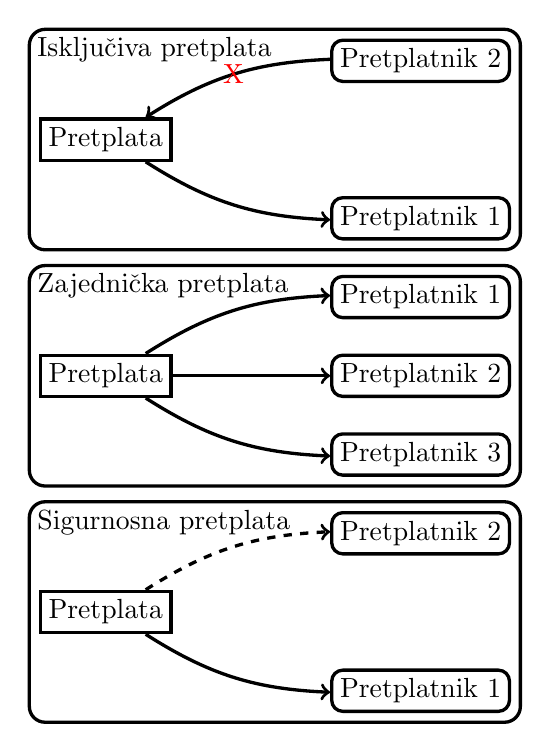
\begin{tikzpicture}[ % has a lot of options; consult the pgf manual
bend angle=15,
long_square/.style={rectangle, draw=black, fill=white, very thick, inner sep=3pt, minimum width=14mm},
rounded_square/.style={rectangle, rounded corners, draw=black, fill=white, very thick, inner sep=3pt, minimum width=14mm},
empty_circle/.style={rectangle, rounded corners=2mm, draw=black, fill=white, very thick, minimum size=4mm},
point/.style={circle, inner sep=0mm},
fit_square/.style={rectangle, rounded corners=2mm, draw=black, very thick},
both_arrow/.style={<->, very thick},
out_arrow/.style={->, very thick},
in_arrow/.style={<-, very thick},
above_edge_text/.style={above, midway, sloped}
]

\node[long_square](sub_1) at (0,0) {Pretplata};
\node[long_square](sub_2) at (0,-3) {Pretplata};
\node[long_square](sub_3) at (0,-6) {Pretplata};

\node[rounded_square](consumer_1) at (4,1) {Pretplatnik 2};
\node[rounded_square](consumer_2) at (4,-1) {Pretplatnik 1};

\node[rounded_square](consumer_3) at (4,-2) {Pretplatnik 1};
\node[rounded_square](consumer_4) at (4,-3) {Pretplatnik 2};
\node[rounded_square](consumer_5) at (4,-4) {Pretplatnik 3};

\node[rounded_square](consumer_6) at (4,-5) {Pretplatnik 2};
\node[rounded_square](consumer_7) at (4,-7) {Pretplatnik 1};

\node[fit_square, fit=(sub_1) (consumer_1) (consumer_2)] (exclusive) {};
\node[anchor=north west] at (exclusive.north west) {Isključiva pretplata};

\node[fit_square, fit=(sub_2) (consumer_3) (consumer_4) (consumer_5)] (shared) {};
\node[anchor=north west] at (shared.north west) {Zajednička pretplata};

\node[fit_square, fit=(sub_3) (consumer_6) (consumer_7)] (failover) {};
\node[anchor=north west] at (failover.north west) {Sigurnosna pretplata};



\draw[out_arrow, text=red](consumer_1) to [bend right] node[midway]{X} (sub_1);
\draw[out_arrow](sub_1) to [bend right] node[above, sloped]{} (consumer_2);

\draw[out_arrow](sub_2) to [bend left] node[auto]{} (consumer_3);
\draw[out_arrow](sub_2) to [] node[auto]{} (consumer_4);
\draw[out_arrow](sub_2) to [bend right] node[auto]{} (consumer_5);

\draw[out_arrow, dashed](sub_3) to [bend left] node[auto]{} (consumer_6);
\draw[out_arrow](sub_3) to [bend right] node[auto]{} (consumer_7);

\end{tikzpicture}

\end{document}